\documentclass[a4paper, czech]{article}

\title{Úloha č.8: Indikátor úrovně s 10 LED AMJ3915SX}
\author{Karolína Šebestová \and Jan Božejovský}
\date{Datum měření: 12.11.2024}

\usepackage[czech]{babel}
\usepackage{indentfirst}
\usepackage{graphicx}
\usepackage{float}
\usepackage[margin=1.5cm]{geometry}
\usepackage{booktabs}
\usepackage{amsmath}
\usepackage{multirow}
\usepackage{caption}
\usepackage{subcaption}

\begin{document}

\maketitle

\section{Teoretický úvod}

\begin{figure}[H]
    \centering
    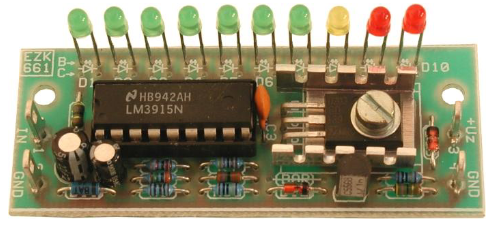
\includegraphics{amj3915sx_foto.png}
    \caption{Fotografie zhotoveného modulu AMJ3915SX}
\end{figure}

AMJ3915SX je monofonní indikátor úrovně (výkonu) s nesymetrickým napájením.
Zapojení indikátoru vychází z doporučeného zapojení integrovaného obvodu LM3915 společnosti National Semiconductor.
Maximální indikované napětí je definováno napěťovým děličem tvořeným odpory R$_2$ a R$_3$.
Integrovaný obvod LM3915 může pracovat buď ve sloupcovém nebo v bodovém režimu.
Pro sloupcový režim musí být pin č. 9 obvodu LM3915 připojen k napájecímu napětí.
Je-li pin č. 9 nezapojen, pracuje obvod v bodovém režimu.
Závislost rozsvěcování LED diod na vstupním napětí je logaritmická, což je pro indikaci výkonu výhodné.

U tohoto modulu je také možno volit buď paralelní nebo sériové zapojení LED.

\begin{figure}[H]
    \centering
    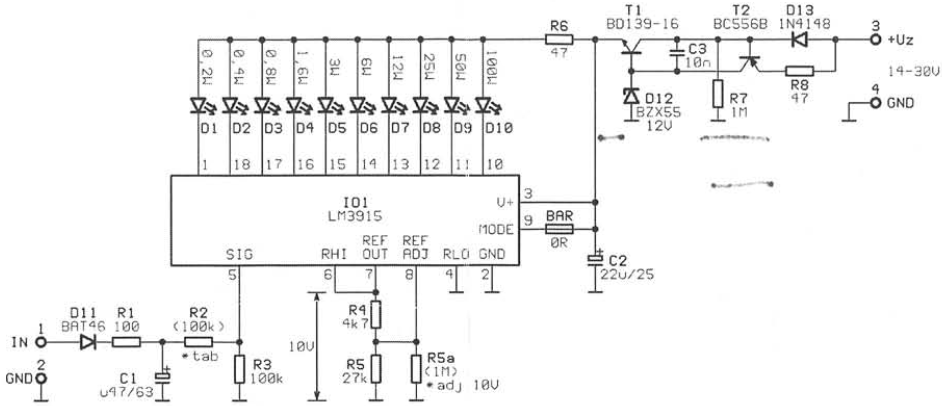
\includegraphics[width=\textwidth]{amj3915sx_schema_paralelni.png}
    \caption{Schéma zapojení modulu s paralelním řazením indikačních LED}
\end{figure}

\pagebreak

\section{Úkoly měření}

\begin{enumerate}
    \item Připojením vstupu obvodu ke generátoru a osciloskopu zjistěte maximální vstupní napětí, tedy napětí pro plnou výchylku indikátoru (včetně červených LED) na několika frekvencích ve slyšitelném pásmu. (Nezapomeňte aktivovat výstup generátoru pomocí stisku tlačítka Channel a volby Output On tlačítkem pod displejem.) V dalších úkolech dbejte na to, aby na vstup obvodu nebylo přivedeno větší napětí.
    \item Změřte hodnoty vstupních sinusových napětí odpovídající rozsvícení jednotlivých LED (od první až po poslední). Toto měření opakujte pro 5 frekvencí přibližně rovnoměrně rozložených (v logaritmickém měřítku) v pásmu 20 Hz – 20 kHz. Na nízkých frekvencích mohou LED blikat, v tom případě považujte blikající LED za rozsvícenou.
    \item Pomocí analyzátoru Bode 100 změřte frekvenční charakteristiky modulu a fáze vstupní impedance (20 Hz – 20 kHz). Změňte amplitudu měřicího signálu (hodnota Level) a posuďte, zda se impedance mění v závislosti na velikosti vstupního napětí.
    \item Zjistěte vliv výchylky indikátoru na proudový odběr z napájecího zdroje. Na displeji napájecího zdroje odečítejte proudový odběr v závislosti na počtu rozsvícených LED.
    \item Prozkoumejte rychlost odezvy měřiče přivedením obdélníkového signálu o nízké frekvenci 1 Hz a amplitudě, kdy se rozsvěcují všechny LED. Na osciloskopu v režimu časové základny Roll (stiskněte tlačítko Horiz a vlevo dole na displeji nastavte Time Mode na Roll) zobrazte napětí na vyvedeném drátku z LED (připojte k němu červenou krokosvorku kabelu k osciloskopu a černou připojte na zem obvodu). Průběh na osciloskopu ve vhodný okamžik zastavte tlačítkem Stop a ze schodovité části průběhu odečtěte doby, za jak dlouho zhasne jedna (doba jednoho „schodu“) a za jak dlouho všechny LED. Z doby sestupné hrany signálu na osciloskopu určete, za jak dlouho se rozsvěcují LED. 
\end{enumerate}

\section{Seznam použitých přístrojů}

\begin{itemize}
    \item Modul indikátoru úrovně AMJ3915SX
    \item Laboratorní napájecí zdroj Agilent E3620A
    \item Laboratorní digitální osciloskop Agilent DSO-X 2002A
    \item Laboratorní signálový generátor
\end{itemize}

\section{Zpracování úkolů}

\subsection{Měření závislosti rozsvícení jednotlivých LED na vstupním napětí (Úkol 2)}

\subsubsection{Tabulky}

\begin{table}[H]
    \catcode`\-=12
    \centering
    \caption{Hodnoty vstupních sinusových napětí odpovídající rozsvícení jednotlivých LED}
    \begin{tabular}{cccccc}
        \toprule
        \multirow{2}{*}{LED} & \multicolumn{5}{c}{$U_{\text{vst}}$ [V]} \\
        \cmidrule(rl){2-6}
            & 20\,Hz    & 100\,Hz   & 1\,kHz  & 10\,kHz & 20\,kHz \\
        \midrule
        1   & 0,80  & 0,87  & 0,85  & 1,03  & 0,80  \\
        2   & 0,95  & 1,06  & 1,06  & 1,09  & 1,05  \\
        3   & 1,31  & 1,54  & 1,39  & 1,34  & 1,36  \\
        4   & 1,91  & 2,03  & 1,85  & 1,85  & 1,83  \\
        5   & 2,41  & 2,57  & 2,45  & 2,41  & 2,41  \\
        6   & 3,26  & 3,32  & 3,34  & 3,28  & 3,24  \\
        7   & 4,46  & 4,62  & 4,46  & 4,46  & 4,49  \\
        8   & 6,47  & 6,87  & 6,31  & 6,23  & 6,19  \\
        9   & 9,10  & 9,20  & 8,80  & 8,80  & 8,67  \\
        10  & 12,20 & 12,80 & 12,10 & 12,10 & 12,00 \\
        \bottomrule
    \end{tabular}
\end{table}

\subsubsection{Grafy}

\begin{figure}[H]
    \centering
    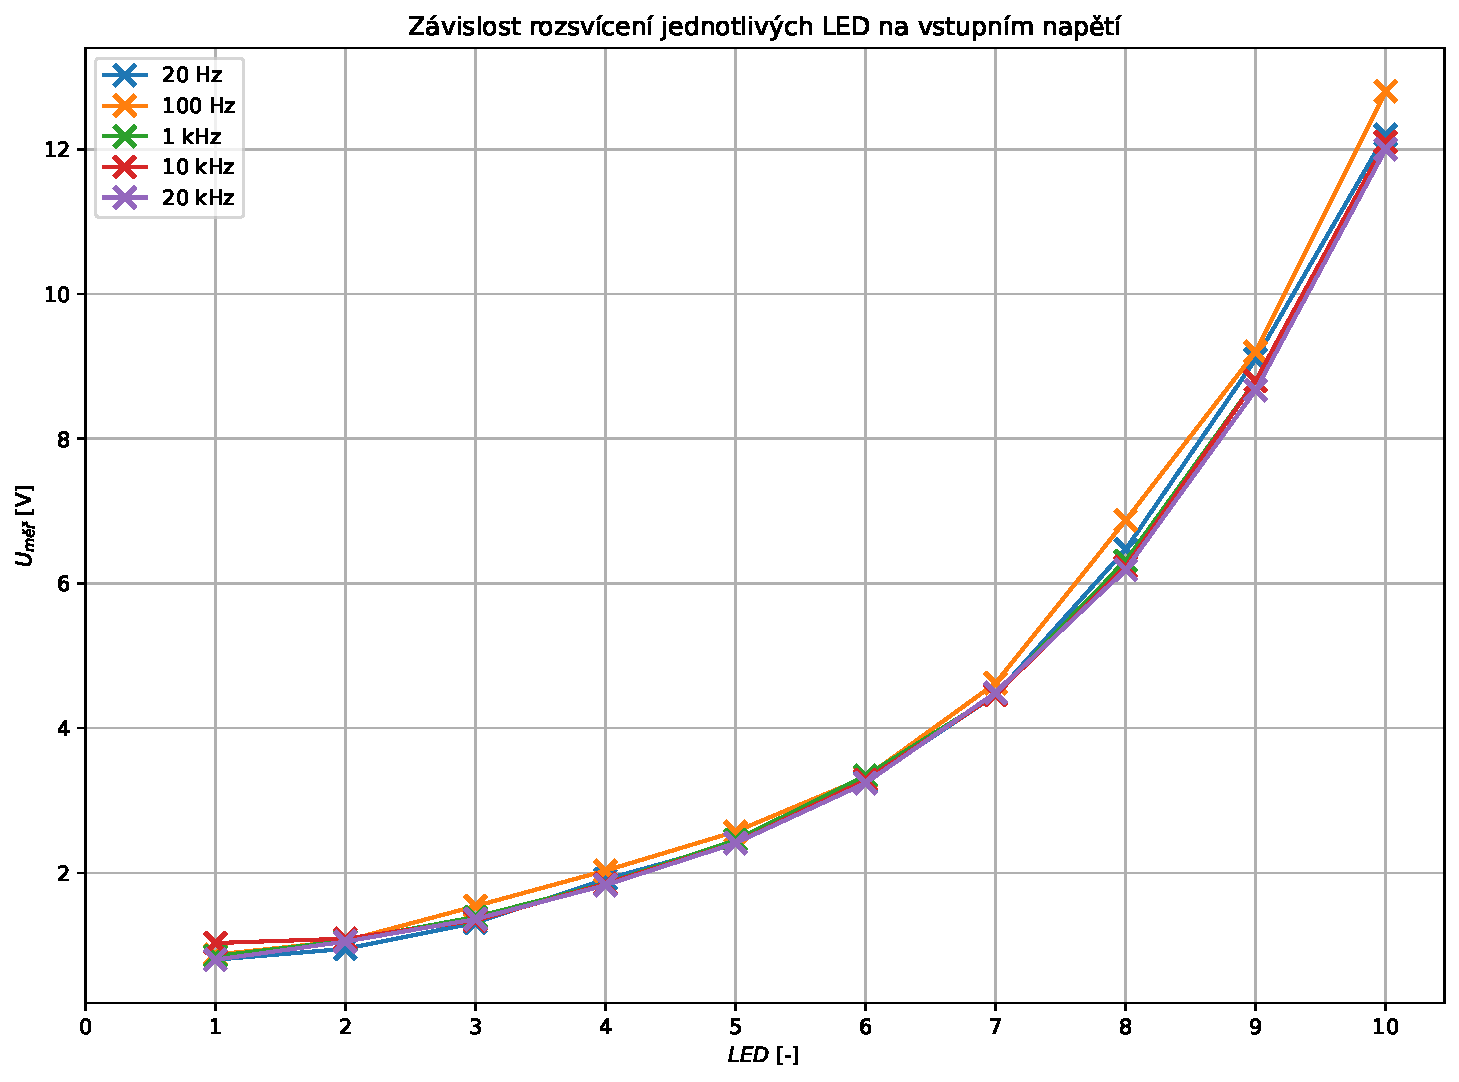
\includegraphics[width=0.8\textwidth]{grafy/graf1.pdf}
    \caption{Závislost rozsvícení jednotlivých LED na vstupním napětí}
\end{figure}

\begin{figure}[H]
    \centering
    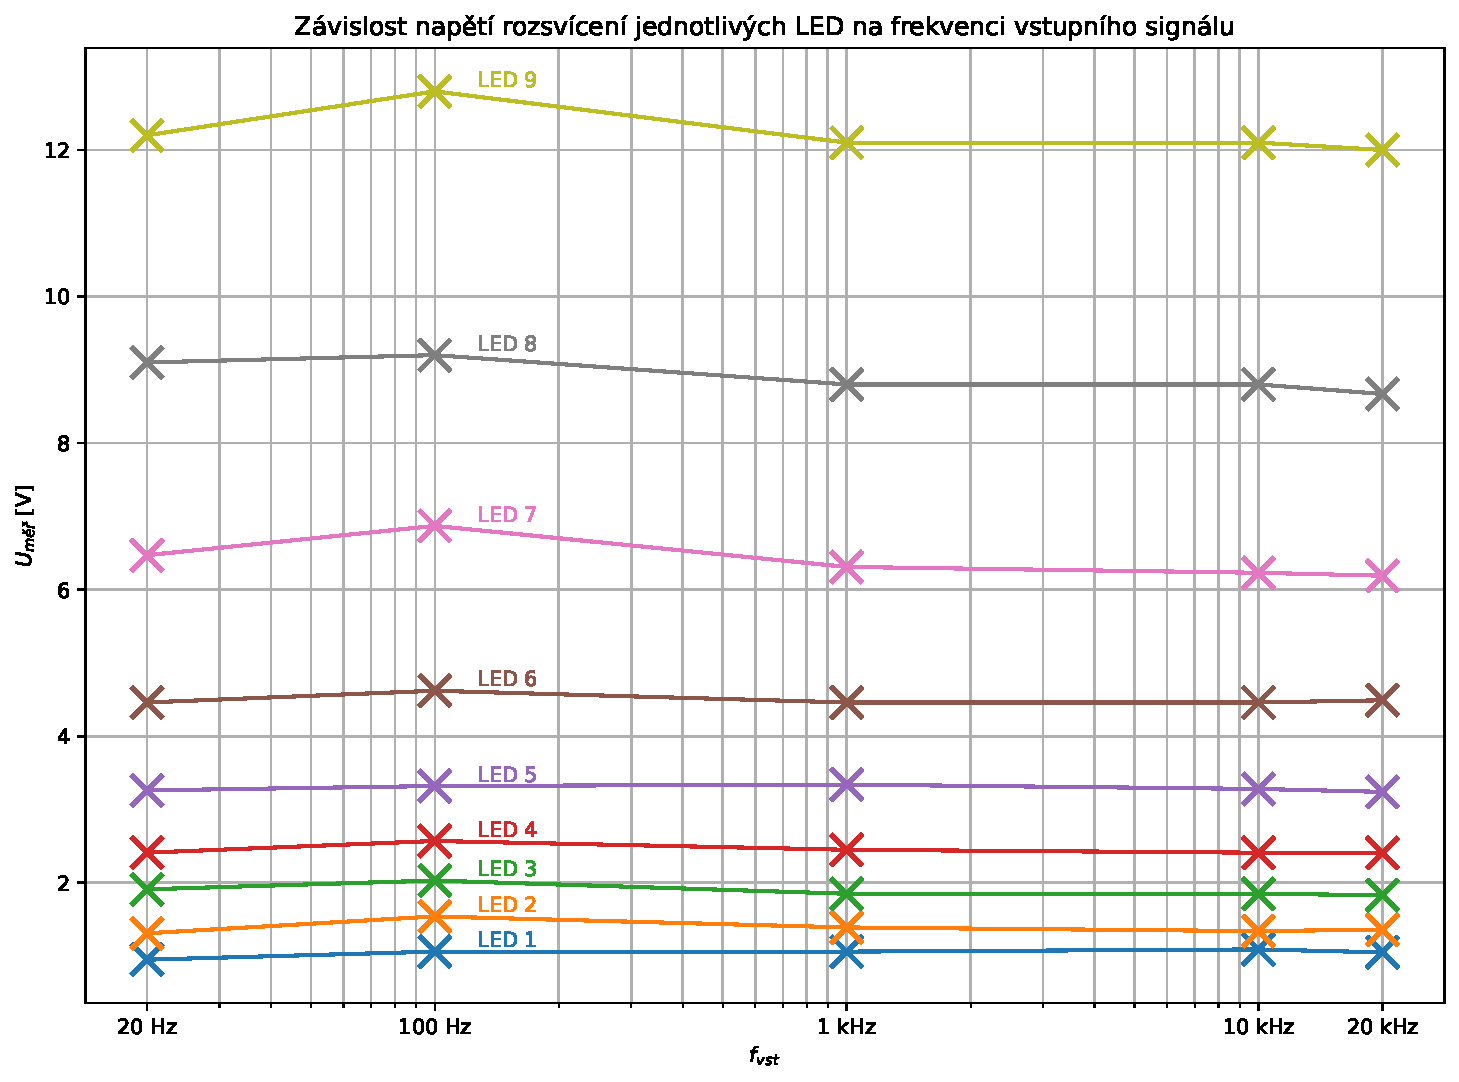
\includegraphics[width=0.8\textwidth]{grafy/graf2.pdf}
    \caption{Závislost napětí rozsvícení jednotlivých LED na frekvenci vstupního signálu}
\end{figure}

\subsection{Měření frekvenční charakteristiky modulu a fáze vstupní impedance (Úkol 3)}

\begin{figure}[H]
    \centering
    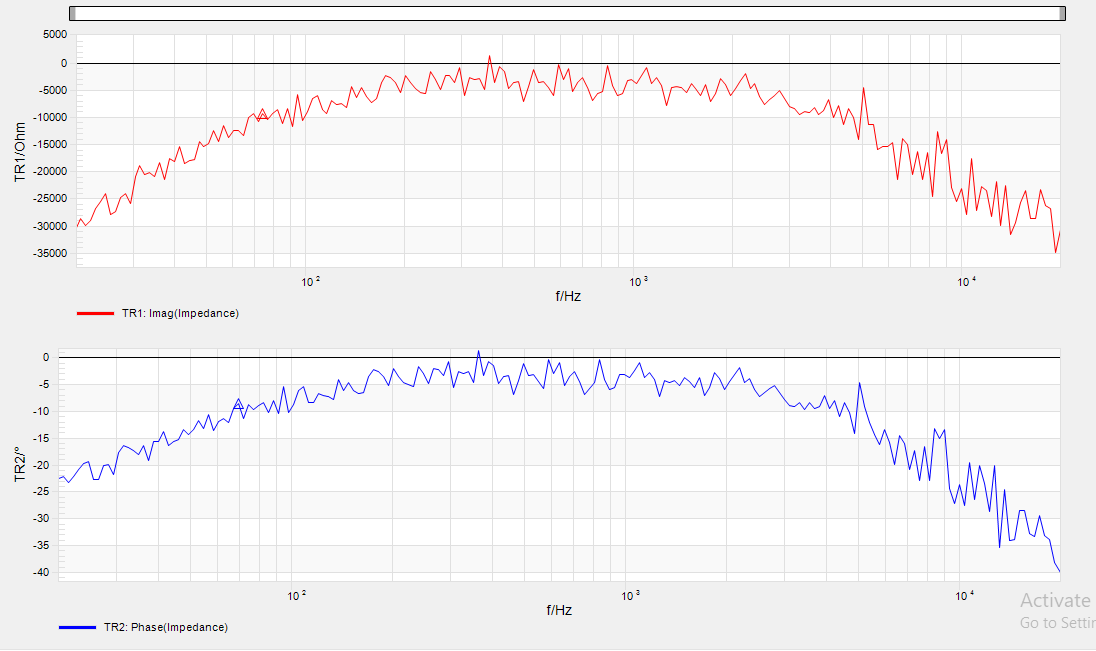
\includegraphics[width=\textwidth]{impedance_uloha8.png}
    \caption{Frekvenční charakteristiky modulu a fáze vstupní impedance při amplitudě výstupní úrovně -3\,dBm}
\end{figure}

\begin{figure}[H]
    \centering
    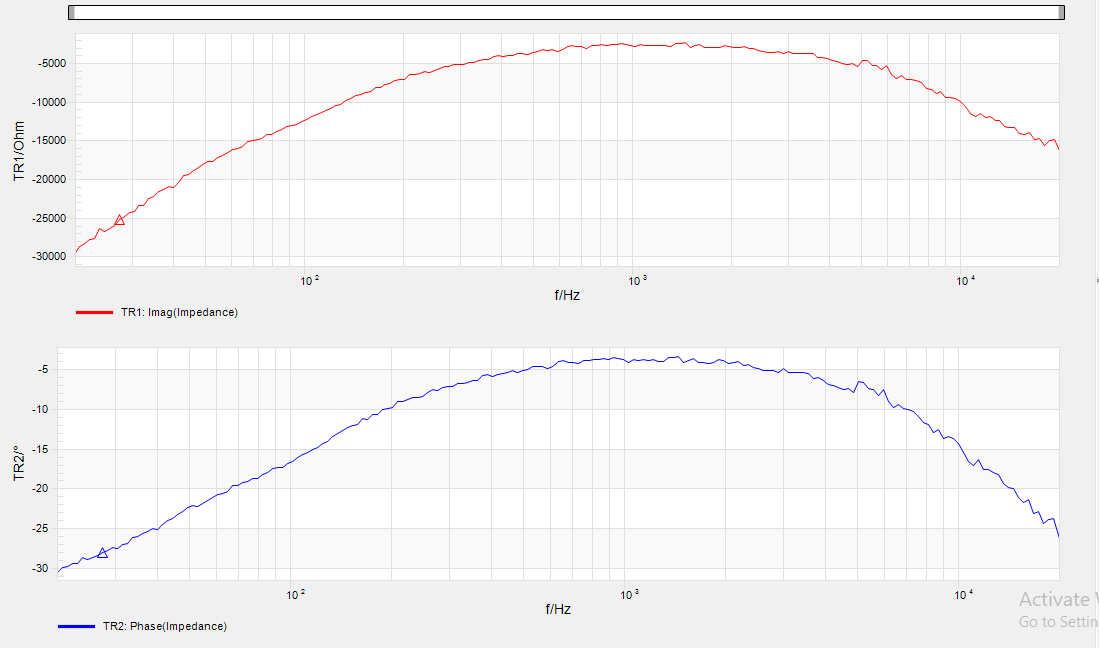
\includegraphics[width=\textwidth]{impedance_13dbm_uloha8.png}
    \caption{Frekvenční charakteristiky modulu a fáze vstupní impedance při amplitudě výstupní úrovně 13\,dBm}
\end{figure}

\subsection{Měření vlivu výchylky indikátoru na proudový odběr z napájecího zdroje (Úkol 4)}

\subsubsection{Tabulky}

\begin{table}[H]
    \catcode`\-=12
    \centering
    \caption{Hodnoty proudového odběru v závislosti na počtu rozsvícených LED}
    \begin{tabular}{ll|cccccccccc}
        \toprule
        LED & [-]              & 1     & 2     & 3     & 4     & 5     & 6     & 7     & 8     & 9     & 10    \\
        \cmidrule(rl){1-12}
        $I_{V_{\text{CC}}}$ & {[}A{]} & 0,011 & 0,017 & 0,024 & 0,030 & 0,036 & 0,042 & 0,048 & 0,054 & 0,060 & 0,065 \\
        \bottomrule
    \end{tabular}
\end{table}

\subsubsection{Grafy}

\begin{figure}[H]
    \centering
    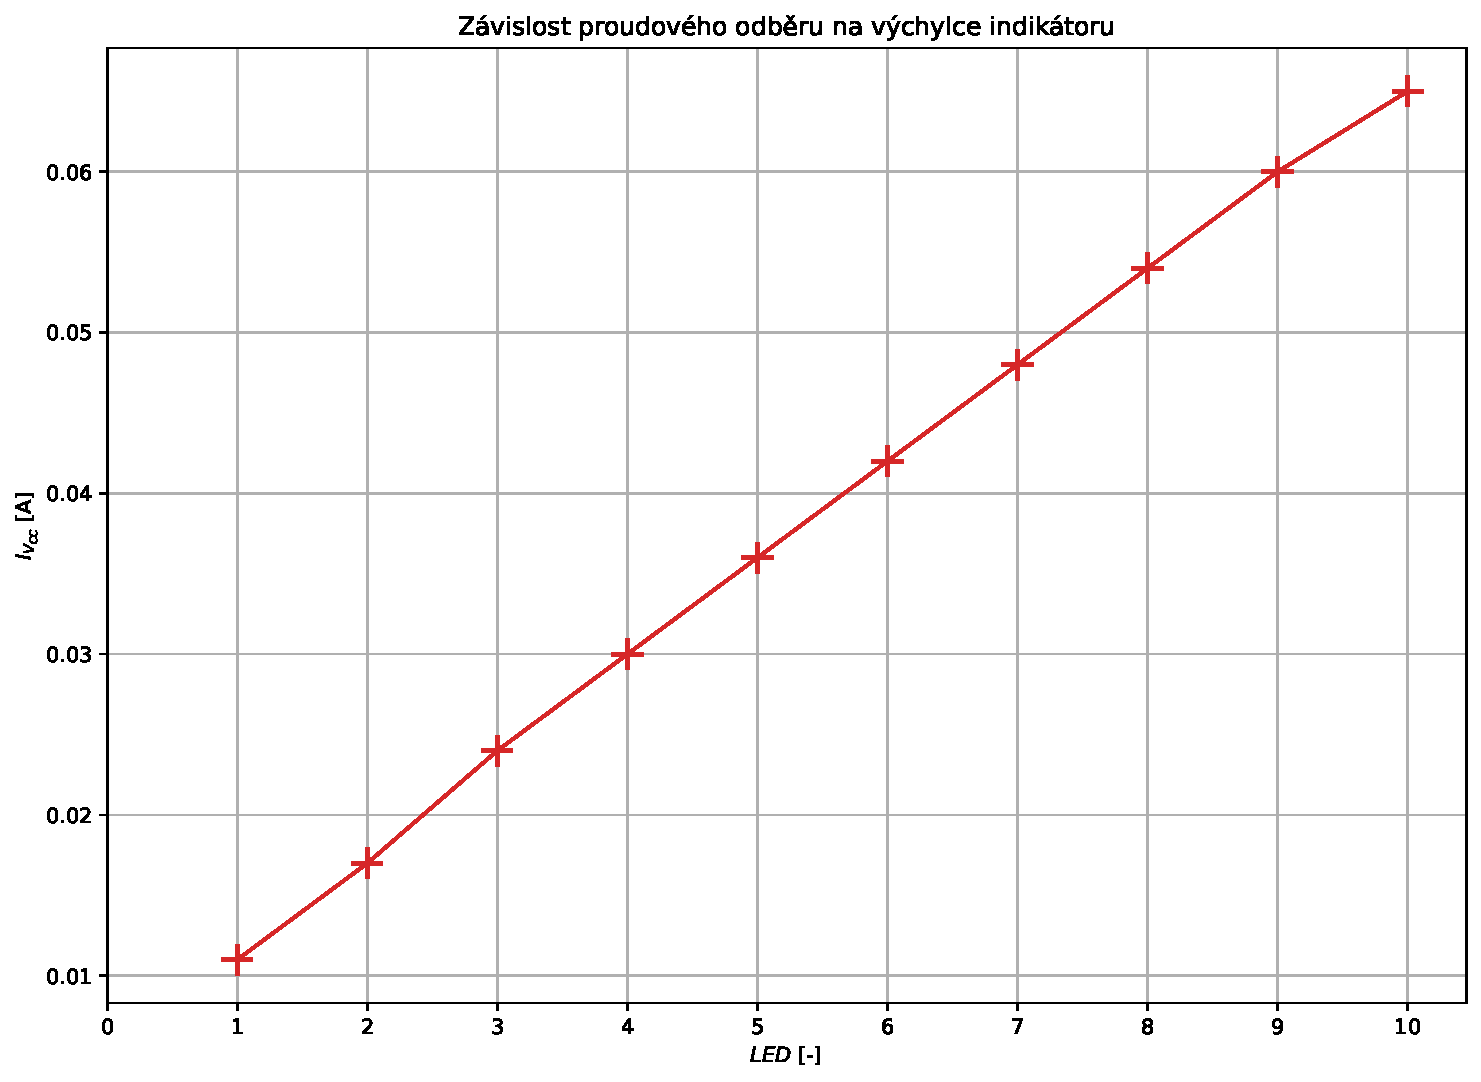
\includegraphics[width=0.8\textwidth]{grafy/graf3.pdf}
    \caption{Závislost velikosti proudového odběru na počtu rozsvícených LED}
\end{figure}

\subsection{Měření rychlosti odezvy měřiče (Úkol 5)}

\subsubsection{Tabulky}

\begin{table}[H]
    \centering
    \caption{Odečtené časové hodnoty rychlosti odezvy měřiče}
    \begin{tabular}{lr}
        \toprule
        Doba zhasnutí jedné LED & 13,2\,ms \\
        Doba zhasnutí všech LED & 121\,ms \\
        Doba rozsvícení LED & 194\,$\mu$s \\
        \bottomrule
    \end{tabular}
\end{table}

\begin{figure}[H]
    \centering
    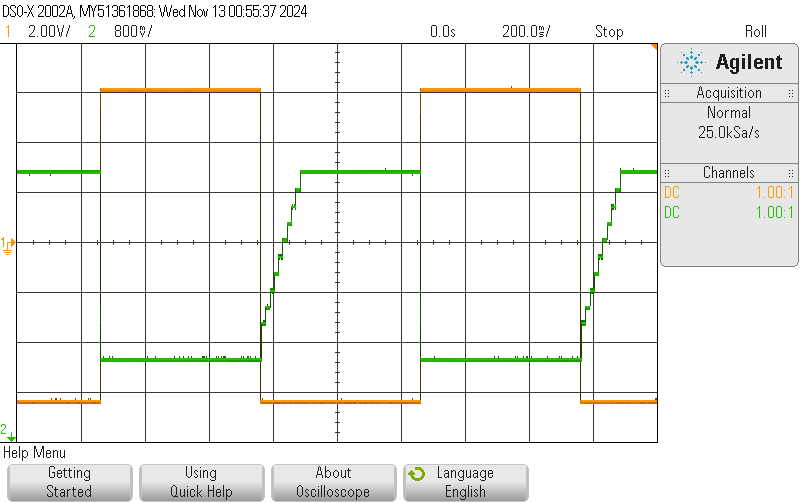
\includegraphics[width=\textwidth]{osciloskop_uloha8.png}
    \caption{Snímek obrazovky osciloskopu během měření zobrazující časový průběh napětí na LED}
\end{figure}

\section{Závěr}

\end{document}